
\documentclass[titlepage]{article}
 \usepackage[utf8]{inputenc}
\usepackage{listings}
\usepackage{float}

\usepackage{graphicx}
\graphicspath{ {imagenes/} }
 \usepackage{xcolor}
 \definecolor{RoyalBlue}{cmyk}{1, 0.50, 0, 0}
 

\lstset{language=Java,
	keywordstyle=\color{RoyalBlue},
	basicstyle=\scriptsize\ttfamily,
	commentstyle=\ttfamily\itshape\color{gray},
	stringstyle=\ttfamily,
	showstringspaces=false,
	breaklines=true,
	frameround=ffff,
	frame=single,
	rulecolor=\color{black}}


 

% Datos de la portada
\begin{document}
	\begin{titlepage}
		\begin{center}
			\vspace*{1cm}
			\date{} % para que no aparezca la fecha la dejo en blanco
			\Huge
			\textbf{Practica 1}
			
			\vspace{0.5cm}
			\LARGE
			T.S.I.
			
			\vspace{1.5cm}
			
			\textbf{José Manuel Pérez Lendínez}
			

			
		\end{center}
	\newpage
	\tableofcontents
	\newpage
	\end{titlepage}
	\section{Descripción General}
	Se ha realizado una mezcla de a* para la parte deliberativa y comportamientos reactivos que harán saltar nuevamente el método de búsqueda a* si se tiene algún problema por el que no se tiene que recalcular la ruta. Para llevar esto acabo tendremos un metodo a* con la siguiente cabezera:
	\newline
	
	\textbf{boolean estrella(stateObs, inicio\_x, inicio\_y, final\_x, fina\_y, mapa)};
	\newline
	
	Le pasamos el mapa como parámetro porque los comportamientos reactivos del agente tendrán la posibilitar de modificar el mapa para cancelar posiciones por las que no puede pasar el agente.
	
	Pasemos al pseudocódigo del metod act.

	\begin{lstlisting}
	if(no hay piedras cayendo){
		//Elimina del path la primera posicion si el avatar avanzo
		eliminarPosicionUtilizada();
		
		int nGema = numero_gemasCogidas();
		
		if(nGemas ditinto a gemasCogidas){
			//El camino se inicializa
			path = new
			gemasCogidas = gemas
		}
		
		if(!hay_Camino){
			if(Si tenemos 9 gemas){
				gemasConseguidas = true
				//Buscamos el portal para salir
				path = obtenerCaminoPortal()
			}else{
				//Pone en path el camino a la gema mas cercana y devuelve un 
				//boleano de si existe camino. Si la mas cercana no lo tiene
				pasa a la siguiente hasta mirar todas
				mapa[][] = obtenerMapa()
				hay_camino = obtenerCaminoGema(avatar, mapa);
				
			}
		}
		
		
	}else{
		//esta parte se utiliza par acuando no tenemos camino y hay 
		//que estar en bucle buscando un camino a la siguiente gema.
		//Se activa normalmente cuando hay piedras que estan callendo
		// y hasta que caen no podemos pasar.
		//Pone en path el camino a la gema mas cercana y devuelve un 
		//boleano de si existe camino. Si la mas cercana no lo tiene
		pasa a la siguiente hasta mirar todas
		mapa[][] = obtenerMapa()
		 hay_camino = obtenerCaminoGema(avatar, mapa);
	}
	
	if(path no es null){
		//obtiene la accion que tiene que realizar el personaje.
		//Avanzar, izquierda, derecha, ...
		siguienteAccion = elegirSiguiente(accion)
		
		//Aqui se dan las opciones reactivas que se explicar mas
		//adelatne por ahor apodnremos la siguiente funcion para
		//tenerlo en cuenta unicamente
		comportamientoReactivo()
		
		//cambiamos la ultima posicon por la actual
		//ultima pos se utiliza en elegirSiguiente accion para
		//elegir que accion tomar
		ultima_pos  = avatar
		
		return siguienteaccion;
	}else{
		return Types.ACTIONS.ACTION_NIL
	}
	\end{lstlisting}
	
	\section{Comportamiento deliberativo}
	
	El pseudocodigo para el algoritmo a* utilizado es el siguiente:
	\begin{figure}[H]
		\centering
		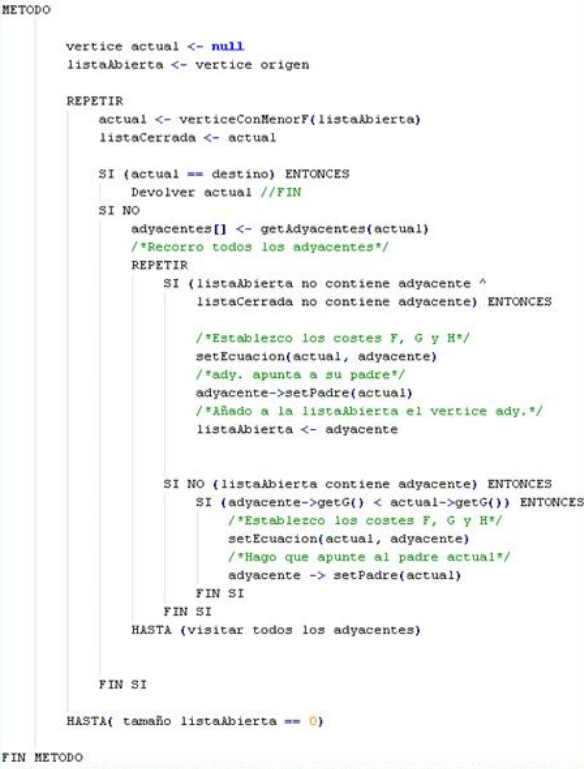
\includegraphics[width=0.7\linewidth]{screenshot001}
		
		\label{fig:screenshot001}
	\end{figure}

	La heuristica empleada es muy simple. Utilizamos el coste hasta el nodo actual (g) + la distancia manhattan (f). 
	Para ir creando el camino he creado una nueva clase llamada NodoEstrella.
	\begin{lstlisting}
		public class NodoEstrella{
			private int g,h,f,x,y;
			public ArrayList<Node> camino;
		}
	\end{lstlisting}
	
	En la variable camino tengo el camino hasta llegar a ese nodo.
	X es la posición x de la casilla e y la posiciona y de la casilla.
	
	La función getAdyacente(actual) devuelve una lista de los nodos que se pueden obtener moviéndonos a derecha,izquierda arriba y abajo. Si en alguna de las posición hay una piedra o un muro ese adyacente no se creara. Actualizo los valores de g h y f a la hora de generar los adyacentes.
	La variable camino la actualizo añadiendo al principio la posición del padre y a continuación concateno con el camino hasta llegar al padre.
	
	La función verticeConMenosF() devuelve el nodo con el menor valor en la variable f.
	
	\section{Comportamiento reactivo}
	Mi comportamiento reactivo tiene 4 reglas.
	\begin{enumerate}
		\item \textbf{Si al cavar hacia arriba me puede caer una piedra en la cabeza.}
		
		\begin{lstlisting}
if(peligroPiedra()){
			
	//marcamos la posicion como si fuera un muro y
	//al realizar la busqueda con el a* no la
	//tendra en cuenta para buscar el nuevo camino
	mapa[][] = obtenerMapa()
	mapa[avatar.x][avatar.y - 1] = muro
		
	bool tenemos_camino = obtenerCaminoGema(avatar, mapa)
	
if(!tenemos_camino){
	//la unica salida es tirando las piedras
	//me tengo que colocar a la derecha o izquierda
	//de la posicion que sin cavar justo debajo de las piedras.
	//de estas forma podre tirarlas
	bool estaColocado = colocarParaCavar();
		
	if(estaColocado){
		siguienteaccion = elegirSiguienteAccion();
	}else{
		siguienteaccion = Types.ACTIONS.ACTION_NIL;
	}
	
		
		
}else{
	if(!hay_camino)
		siguienteaccion = elegirSiguienteAccion()
	}else{
		siguienteaccion = Types.ACTIONS.ACTION_NIL;
	}
		
}
		\end{lstlisting}
		\item \textbf{Si me encuentro una piedra de frente:}
		Este caso es mas simple unicamente llamo al buscarGema o buscarPortal dependiendo del numero de gemas que tenga para buscar un nuevo camino.Este caso se puede dar cuando has tirado piedras y no se usaron para crear el camino anterior.
		
		\begin{lstlisting}
if(piedraDelante())
	//gemas conseguidas nos dice si tenemos o no todas las gemas
	if(!gemasConseguidas) {
		mapa[][] = obtenerMapa()
		obteneCaminoGema(mapa);
	}else{
		mapa[][] = obtenerMapa()
		obteneCaminoPortal(mapa);
	}
}
\end{lstlisting}
		\item \textbf{Si tengo un bicho en alguna de las dos posiciones contiguas a la actual que tomare por el camino dado en el a*: }
		En este caso lo que voy mirando es si en las dos siguientes posiciones del camino tengo o no un bicho, en caso de tenerla en una de las dos se marca esa casilla como no valido y lo intento evitar para no chocar con el. Uso las dos posiciones siguientes del camino porque ne algunos mapas usar una u otra puede mejorarte mucho. Con esto consigo tener lo mejor de las dos partes. Después de realizar pruebas con las tres combinaciones posibles esta fue la que mejor resultados me dio.
		
\begin{lstlisting}
if(peligroBicho(0)) {
	mapa[][] = obtenerMapa()
	mapa[path[0].x][path[0].y] = Types.wall
	
	if(!gemasConseguidas) {
		obteneCaminoGema(mapa);
	}else{
		obteneCaminoPortal(mapa);
	}
}else if(peligroBicho(1)){
	mapa[][] = obtenerMapa()
	mapa[path[1].x][path[1].y] = Types.wall
	
	if(!gemasConseguidas) {
		obteneCaminoGema(mapa);
	}else{
		obteneCaminoPortal(mapa);
	}
}

\end{lstlisting}	
	\end{enumerate}
	
	
	
	
	
	


	
	
	
	
	
	
	
	
 
  
\end{document}